\message{ !name(main.tex)}\documentclass{easychair}

\usepackage{url}
\usepackage{xspace}
\usepackage{xparse}
\usepackage{color}
\usepackage{amsmath, amsfonts, amssymb}
\usepackage{stmaryrd}
\usepackage{mathrsfs}
\usepackage{mathtools}
\usepackage{array}
\usepackage[ruled,vlined,linesnumbered]{algorithm2e}
\usepackage{enumitem}
\usepackage{endnotes}
\usepackage{hyperref}
\usepackage{bussproofs}
\usepackage{subcaption}

\usepackage{marvosym}

\def\B{\mathcal{B}}
\def\C{\mathcal{C}}
\def\D{\mathcal{D}}
\def\E{\mathcal{E}}
\def\F{\mathcal{F}}
\def\G{\mathcal{G}}
\def\I{\mathcal{I}}
\def\L{\mathcal{L}}
\def\M{\mathcal{M}}
\def\O{\mathcal{O}}
\def\P{\mathcal{P}}
\def\Q{\mathcal{Q}}
\def\R{\mathcal{R}}
\def\S{\mathcal{S}}
\def\T{\mathcal{T}}
\def\U{\mathcal{U}}
\def\V{\mathcal{V}}
\def\W{\mathcal{W}}
\def\X{\mathcal{X}}

\def\Cf{\mathfrak{C}}
\def\Df{\mathfrak{D}}
\def\Ifr{\mathfrak{I}}
\def\Sf{\mathfrak{S}}


\newcommand{\dom}{\mathit{dom}}
\newcommand{\ran}{\mathit{ran}}
\newcommand{\FV}{\text{FV}}

\newcommand{\lang}{\mathscr{L}}

\newcommand*\red[1]{\textcolor{red}{#1}}
\newcommand*\blue[1]{\textcolor{blue}{#1}}

%%% Local Variables:
%%% mode: latex
%%% TeX-master: t
%%% End:

\usepackage{xspace}
\usepackage{mathtools}
\usepackage{dashrule}

\newcommand{\verit}{{\sf veriT}\xspace}
\newcommand{\veriT}{\verit}
\newcommand{\ematch}{\emph{E}-matching}
\newcommand{\dpllt}{DPLL($\T$)}
\newcommand{\ccfv}{\textsc{CCFV}}
\def\sup{\textsc{Sup}}

% *************** For CCFV

\newcommand{\pabs}[1]{#1^{\emph{p}}}
\newcommand{\gabs}[1]{#1^{\emph{g}}}

\newcommand{\bottop}{\mathclap{\raise.1ex\hbox{\hspace{2.9mm}\scalebox{.9}{$\top$}}}{\scalebox{.9}{$\bot$}}}

\DeclareDocumentCommand{\mymodels}{O{} D(){\hspace{0.75ex}}}{\mathrel{{\mathclap{\raise1.1ex\hbox{\hspace{7.5mm}\scalebox{.75}{#1}}}{\models_{\msub{#2}}}}}}
\def\msub#1{\raisebox{-.5ex}{\hbox{\scriptsize $#1$}}}

% \newcommand{\fuzzyeq}{\mathrel{{\mathclap{\rotatebox{45}{\raise-1.8ex\hbox{\hspace{7.5mm}{\hdashrule{3ex}{1.5pt}{3pt}}}}}{\simeq}}}\vspace{-1.8ex}}

\newcommand{\fuzzyeq}{\mathrel{{\mathrlap{\simeq}{\hspace{.3ex}\raise-.5ex\hbox{\rotatebox{64}{\hdashrule{3ex}{.45pt}{1pt}}}}}}}


\newcommand\mgr[1][]{\mathrel{{\mathclap{\raise1.25ex\hbox{\hspace{7.5mm}\scalebox{.75}{g}}}{\models_{\msub{#1}}}}}}
\newcommand\mb[1][\hspace{.5ex}]{\mathrel{\clap{\raise.9ex\hbox{\hspace{7.5mm}\scalebox{.75}{b}}}{\models_{\msub{#1}}}}}

\newcommand{\leqdot}{\mathbin{\clap{\raise.1ex\hbox{\hspace{4.0mm}\scalebox{1.25}{$\cdot$}}}{\leq}}}

% \newcommand\ceq  {\mathbin{\clap{\raise1.0ex\hbox{\hspace{3.2mm}\scalebox{.75}{$\mathbf{*}$}}}{=}}}
% \newcommand\cneq {\mathbin{\clap{\raise1.0ex\hbox{\hspace{3.2mm}\scalebox{.75}{$\mathbf{*}$}}}{\neq}}}
\newcommand\ceq  {\approx_{\mathfrak{C}}}
\newcommand\cneq  {\not\approx_{\mathfrak{C}}}

\newcommand{\eqs}{\Cf}
\newcommand{\dis}{\Df}
\newcommand{\cinst}{\Ifr}

% \newcommand{\finstf}[2][]{\textsc{GetFInst}\ #1 #2}
\DeclareDocumentCommand{\suni}{O{\Q^M} g o}
{%
  \IfNoValueTF{#2}
  {%
    \textsc{U}^{#1}
  }%
  {%
    \IfNoValueTF{#3}
    {%
      \textsc{U}^{#1}_{r_#2}
    }%
    {%
      \textsc{U}^{#1}_{r_#2, c_#3}
    }%
  }%
}%

\DeclareDocumentCommand{\uni}{O{\approx} m O{\sigma} O{\L}}{\inneruni(#4, #3, #2,#1)}
  \def\inneruni(#1,#2,#3,#4,#5){{\textsc{Unify}\ #1\ #2\ #3#5 #4}}

\newcommand{\cs}[1][\psi]{\C_{#1}}
\newcommand\cfs[1][\mathbf{x}]{\Delta_{#1}}
% \newcommand\cfs[1][\mathbf{x}]{\Delta_{#1}}
\newcommand{\rep}[1]{\llbracket #1\rrbracket}
\newcommand{\cls}[1]{[#1]}
\newcommand\ecc[1][\psi]{\textsc{E}^{#1}}


\DeclareDocumentCommand{\getcsubs}{O{\T} m O{\qg{\forall,x,\psi}}}{\textsc{GetSubs}\ #1\ #2\ #3}
\DeclareDocumentCommand{\insts}{O{\T} m}{\innerinsts(#1,#2)}
  \def\innerinsts(#1,#2,#3){\textsc{Inst}\ #1\ #2\ #3}

\DeclareDocumentCommand{\ccapp}{ O{f^*} m}{#1(\mapls[\rep]{#2})}

% *************** For E-unification

\newcommand{\euni}{\emph{E}-unification}
\newcommand{\eunif}{\emph{E}-unifier}
\newcommand{\eunifs}{\emph{E}-unifiers}

%%% Local Variables:
%%% mode: latex
%%% TeX-master: t
%%% End:

% *************** Math writing

% macro for building mappings: tuples for the maps (the n-1 first
% elements are mapped to the n-th element)
\ExplSyntaxOn
\NewDocumentCommand{\mapls}{ O{\overline} m }
 {
  % transfer control to an internal fun
  \porst_mylist:nn { #1 } { #2 }
 }

\seq_new:N \l__porst_list_items_seq
\seq_new:N \l__porst_list_output_seq

\cs_new_protected:Npn \porst_mylist:nn #1 #2
 {
  % clear the output sequence
  \seq_clear:N \l__porst_list_output_seq
  % split the input at ,
  \seq_set_split:Nnn \l__porst_list_items_seq { , } { #2 }
  % append each item to the output sequence
  \seq_map_inline:Nn \l__porst_list_items_seq
   {
    % #1 is the given argument, ##1 represents the current item
    \seq_put_right:Nn \l__porst_list_output_seq { #1 { ##1 } }
   }
  % output the sequence with something between items
  \seq_use:Nn \l__porst_list_output_seq {,~} % adjust
 }
\ExplSyntaxOff

\newcommand{\val}[2][\mbox{\scriptsize\scalebox{0.75}[1.0]{$\M$}}]{\llbracket #2\rrbracket^{#1}}
\def\th#1{\text{Th}(#1)}
\def\mod#1{\text{Mod}(#1)}
% \DeclareDocumentCommand{\terms}{ O{} O{}}{\mathbf{T}^{#1}_{#2}}
\DeclareDocumentCommand{\terms}{ O{} O{}}{\mathbf{T}_{#2}(#1)}
\DeclareDocumentCommand{\sel}{ m }{\textsc{sel}(#1)}
\DeclareDocumentCommand{\enum}{ O{n} m O{,} O{} O{1}}{#2_#5#4#3\dots #3#2_{#1}#4}
\DeclareDocumentCommand{\benum}{ O{n} m O{\mapsto} O{} O{,} O{1}}{\innerbenum(#2,#3,#6,#4)#5\dots #5\innerbenum(#2,#3,#1,#4)}
  \def\innerbenum(#1,#2,#3,#4,#5){#1_{#4}#3 #5{#2_{#4}}}
\DeclareDocumentCommand{\bfenum}{O{\mapsto} m}{\innerbfenum(#2,#1)}
  \def\innerbfenum(#1,#2,#3){\mathbf{#1}#3 \mathbf{#2}}
\DeclareDocumentCommand{\fapp}{ O{f} m O{n} O{,} O{(} O{)}}{#1#5#2_1#4\dots #4#2_{#3}#6}
\DeclareDocumentCommand{\ovapp}{ O{f} m}{#1(\overline{#2})}
\DeclareDocumentCommand{\bfapp}{ O{f} m}{#1(\mathbf{#2})}
\DeclareDocumentCommand{\ovfapp}{ O{f} m}{#1(\overline{#2})}
\DeclareDocumentCommand{\map}{ O{f} m m O{f} O{n}}{#1(#2{#3_1},\dots ,#2{#3_{#4}})}

\DeclareDocumentCommand{\emod}{ O{x} O{d}
  O{\M}}{#3_{\mathbf{#1}\mapsto\mathbf{#2}}}

\newcommand{\qgo}[1]{\innerqgo(#1)}
    \def\innerqgo(#1,#2,#3){#1 #2_1\dots #2_n.{#3}}
\def\qg#1{\innerqg(#1)}
    \def\innerqg(#1,#2,#3){#1\mathbf{#2}.{#3}}

\renewcommand{\sin}{\hspace{.1ex}\in\hspace{.3ex}}
\newcommand{\scomma}{,\hspace{.3ex}}

%%% Local Variables:
%%% mode: latex
%%% TeX-master: t
%%% End:

\usepackage{enumitem}
\usepackage{changepage}

\newcommand{\smarginpar}[1]{\marginpar{\scriptsize{#1}}}

% **************** Chapter that does not count and resets sections
\newcommand{\revchapter}[2][]{
    \setcounter{section}{0}
    % \chapter*{#2}
    \chapter[#2: #1]{#2\\[2ex]\Large#1}
}

% **************** Centered itemize/enumeration

\newlength{\mylongest}
% \setlength{\mylongest}{\widthof{The longest label I will need}}
\setlength{\mylongest}{\widthof{Gim}}
\addtolength{\mylongest}{\labelsep}
\SetLabelAlign{CenterWithParen}{\makebox[\mylongest]{(#1)}}

\newenvironment{enumcenter}{
\begin{enumerate}[style=unboxed,align=CenterWithParen,labelwidth=\mylongest,leftmargin=!,label=\textbf{\roman*}]
}{
  \end{enumerate}
}

% **************** Digressions as blocks right shifted and with text guards

\makeatletter
\newenvironment{digression}[1][Beginning of digression]{\par
\pushQED{\emph{End of digression}}%
\normalfont \topsep6\p@\@plus6\p@\relax
\trivlist
\item\relax
{\itshape
#1\@addpunct{.}}\hspace\labelsep\ignorespaces \\[1ex]
\begin{adjustwidth}{2ex}{0pt}
}{%
\end{adjustwidth}
\ \\\popQED\endtrivlist\@endpefalse
}
\makeatother

%%% Local Variables:
%%% mode: latex
%%% TeX-master: t
%%% End:

\usepackage{enumitem}
\usepackage{array}
\usepackage{multirow}

% ***************** tables

% counting lines/columns (see
% http://tex.stackexchange.com/questions/65649/counters-for-use-in-array-tabular-cells)

\newcounter{tabrow}
\newcounter{fdef}

% Environment for functions definitions with parameterized number of displaymath
% columns after labelled one; counter is set to optional arg, default 0
\newenvironment{funcdef}[2][0]
{
\setcounter{fdef}{#1}
\def\arraystretch{1.2}
\begin{center}
\begin{tabular}{>{(\refstepcounter{fdef}\thefdef)}r*{#2}{>{$\displaystyle} l <{$}}}
}
{
\end{tabular}
\end{center}
}

\newenvironment{conds}[2][0]
{
\setcounter{fdef}{#1}
\def\arraystretch{1.2}\small
% \begin{tabular}{>{(\refstepcounter{fdef}\thefdef)}r*{#2}l}
\begin{tabular}{>{(\refstepcounter{fdef}\roman{fdef})}c*{#2}l}
}
{
\end{tabular}
}


% Column that takes width (left justified): L{1cm}, e.g.
\newcolumntype{L}[1]{>{\raggedright\arraybackslash$} p{#1} <{$}}

% Column with math mode in displaystyle
\newcolumntype{F}[1]{>{$\displaystyle} #1 <{$}}

% Allows to break like in cell; first arg is $t,b,c$, for alignment with other cells
\newcommand{\specialcell}[2][c]{%
  \begin{tabular}[#1]{@{}l@{}}#2\end{tabular}}

%%% Local Variables:
%%% mode: latex
%%% TeX-master: t
%%% End:

\usepackage[ruled,vlined,linesnumbered]{algorithm2e}

% *************** algorithm2e

% Do not make stuff italic
\SetArgSty{textrm}
\SetFuncSty{textrm}
% \SetProcNameSty{textrm}

% space between and after float
% \setlength{\intextsep}{1\baselineskip}

% do while construct: do{<end condition>}{<body>}
\SetKwRepeat{Do}{do}{while}

% \SetKwIF{Let}{}{}{let}{\{}}
% \SetKwIF{If}{ElseIf}{Else}{if}{\{}{elif}{else\{}{}%

% match block; use \lCase for inline case
\SetKwSwitch{Match}{Case}{Other}{match}{:}{}{otherwise}{}

\SetKwSwitch{Let}{Case}{Other}{let}{in}{}{otherwise}{}

% match function block; works the same way
\SetKwSwitch{MatchFunc}{Case}{Other}{func}{:}{}{otherwise}{}

% general algorithm construct: \alg{\function{<args>}}{<body>}{???}
\SetKwProg{alg}{proc}{}{}

\SetKwProg{func}{func}{}
% \SetKw{func}{func}{}


\let\oldnl\nl% Store \nl in \oldnl
\newcommand{\nonl}{\renewcommand{\nl}{\let\nl\oldnl}}% Remove line number for one line

% put comments in small colored font; \tcp* for inline, \tcc for block
\newcommand\mycommfont[1]{\footnotesize\ttfamily\textcolor{black}{#1}}
\SetCommentSty{mycommfont}

% defines algorithm environment to put caption below while still ruled
\makeatletter
\newenvironment{Ualgorithm}[1][htpb]
  {\def\@algocf@post@ruled{\kern\interspacealgoruled\hrule  height\algoheightrule\kern3pt\relax}%
    \def\@algocf@capt@ruled{under}
    \begin{algorithm}[#1]}
  {\end{algorithm}}
\makeatother

\renewcommand*{\algorithmcfname}{Fig.}

%%% Local Variables:
%%% mode: latex
%%% TeX-master: t
%%% End:

\usepackage{tikz-qtree}

\usetikzlibrary{automata, arrows}

\makeatletter
\newcommand*\ifcounter[1]{%
  \ifcsname c@#1\endcsname
    \expandafter\@firstoftwo
  \else
    \expandafter\@secondoftwo
  \fi
}
\makeatother

% Very basic; draws arrows between the source and all targets; only one
% source allowed
\newcommand\source[2]{%
  \tikz[remember picture,baseline,inner sep=0pt] {%
    \node [name=source-#1,anchor=base]{$#2$};
  }%
  % \newcounter{target#1}
  % \setcounter{target#1}{0}
}

\newcommand\target[2]{%
    \tikz[remember picture,baseline,inner sep=0pt] {%
        \node [name=target-#1-\arabic{target#1},anchor=base]{$#2$};
    }%
    \stepcounter{target#1}%
}

% #1 - how sharp is the angle
% #2 - identifier of the connection
% #3 - label of connection
% #4 - where the label stays vertically
% #5 - where the label stays horizontally
% #6 - whether it bends up or down
% #7 - whether it connects top or bottom
\DeclareDocumentCommand{\drawconnections}{o m m O{0} O{.5} O{left} O{north}}
{%
  \IfNoValueTF{#1}
  {%
    \tikz[remember picture, overlay, -latex] {
        \foreach \i [evaluate=\i as \n using int(\i-1)] in {1,...,\value{target#2}} {
          \draw[bend #6] (source-#2.#7) to node[auto, yshift=#4,pos=#5] {{\scriptsize \textcolor{blue}{#3}}} (target-#2-\n.#7);
        }
    }
  }%
  {%
    \tikz[remember picture, overlay, -latex] {
        \foreach \i [evaluate=\i as \n using int(\i-1)] in {1,...,\value{target#2}} {
          \draw[bend #6=#1] (source-#2.#7) to node[auto, yshift=#4, pos=#5] {{\scriptsize \textcolor{blue}{#3}}} (target-#2-\n.#7);
        }
    }
  }%
}%

% Allows fancier stuff
\newcommand{\tikzmark}[1]{\tikz[overlay,remember picture] \node (#1) {};}
\newcommand{\DrawBox}[2]{%
  \begin{tikzpicture}[overlay,remember picture]
    \draw[-,shorten >=5pt,shorten <=5pt,out=70,in=130,distance=0.5cm,#1] (c.north) to (d.north);
    \draw[-,shorten >=5pt,shorten <=5pt,out=50,in=140,distance=0.3cm,#2] (a.north) to (b.north);
  \end{tikzpicture}
}

% \newcommand{\DrawBox}[4]{%
%   \begin{tikzpicture}[overlay,remember picture,-latex,shorten >=5pt,shorten <=5pt,out=70,in=130]
%     \draw[distance=0.45cm,#1] (a.north) to (b.north);
%     \draw[distance=0.65cm,#2] (a.north) to (c.north);
%     \draw[distance=0.9cm, #3] (a.north) to (d.north);
%     \draw[distance=1.1cm, #4] (a.north) to (e.north);
%   \end{tikzpicture}
% }

%%% Local Variables:
%%% mode: latex
%%% TeX-master: t
%%% End:


\title{Efficient Instantiation Techniques in SMT (Work In Progress)}
\titlerunning{Efficient Instantiation Techniques in SMT}

\author{Haniel Barbosa}

\authorrunning{Haniel Barbosa}

\institute{LORIA, INRIA, Universit\'{e} de Lorraine, Nancy, France
  \\ \email{Haniel.Barbosa@inria.fr}
}

\begin{document}

\message{ !name(main.tex) !offset(-3) }


\maketitle

\begin{abstract}
In SMT solving one generally applies heuristic instantiation
techniques to handle quantified formulas, which may lead to many
spurious instances interfering with the solver's performance.
Therefore deriving both fewer and more meaningful instances as well
as eliminating or disregarding those not significant for the solving
are desirable features for dealing with first-order problems.

This paper presents preliminary work on introducing sorting criteria
for instances derived through heuristics and the implementation of an
incomplete goal-oriented instantiation technique for SMT. Our
experiments show that while the latter improves performance in general
the former is highly dependent on the problem structure, but its
combination with the classic strategy leads to competitive results
w.r.t. state-of-the-art SMT solvers in several benchmark libraries.
\end{abstract}

\section{Introduction}
\label{sec:intro}

SMT solvers (see~\cite{Barret2009} for a general presentation of SMT)
are extremely efficient at handling large ground formulas with
interpreted symbols, but they still struggle to manage quantified
formulas.  Quantified first-order logic is best handled with
resolution-based theorem
proving~\cite{Bachmair1994,Nieuwenhuis2001-har}. Although there are
first attempts to unify SMT and resolution~\cite{deMoura2008}, the
main approach used in SMT is still \emph{instantiation}: quantified
formulas are freed from quantifiers and refuted with the help of
decision procedures for ground formulas.

The more common strategy for finding instances


MBQI and conflicting instances are both goal-oriented. We implement
the latter through CCFV

Even though such techniques as
{\ematch}~\cite{Detlefs2005} and model based quantifier instantiation
(MBQI)~\cite{Ge2009} have been used successfully in state-of-the-art
solvers, there are still far more instances produced than would actually be
needed.  Reynolds et al.~\cite{Reynolds2014} present an alternative
approach: instances are generated such that they are conflicting, by
construction, with the ground context produced by the solver.  This provides a
strong advantage due to its finer instantiation guideline: less instances
are needed to prove a formula unsatisfiable, as their experimentation data
indicates.

Since their method is restricted to problems in pure first-order logic with
equality, it has strong reminiscence of the (non-simultaneous) rigid {\euni}
problem.  Unifying two expressions with free variables modulo a set of equations
is equivalent, as shown in~\cite{Tiwari2000}, to finding instances
conflicting with a ground context.  In this preliminary work we try to exploit
this relation while revisiting the technique: defining an enhanced version of
the classic congruence closure procedure capable of handling \emph{free
  variables} unification accordingly.  We aim for a better integration of ground
conflicting instance generation and {\ematch}~techniques within core SMT
algorithms (namely the congruence closure decision procedure), with MBQI being
used as last resort.

Using incomplete goal-oriented techniques, if fast, can lead to fewer,
and more meagninful, instances and significant performance
improvements, but the backbone of the search still relies on the
heuristics. In order to mitigate the negative impact of such instances
we introduce sorting criteria according to their usefulness for the
SAT solver

Reynolds \emph{et al.} have shown that by first deriving instances
that refute the current ground context, fewer and more meaningful, and
only when failing resorting back to heuristics leads to significant
perform enhancements.

I want to combine both because models needed to be refuted fast and we
still don't have a complete goal-oriented method. Let alone the fact
that when theories besides equality are involved, as in the rule
rather than the exception in SMT, no ilusion of completeness can be
attained.

Through heuristic instantiation based of pattern-matching SMT solvers
derive instances in a ``no-goal oriented'' fashion: instances are
generated because it's possible, not with a goal in mind. However,
unlike other no-goal oriented techniques such as \emph{Superposition}
there are no straightforward redundancy criteria for the elimination
of derived instances in SMT solving. By keeping track of how the SAT
solver handles the produced instances\smarginpar{Usefulness and at
  which point in the decision tree they were generated.} we try to
compensate for the lack of such criterea for those instances.

People that talked about this in way or another: using two SAT solvers~\cite{Leino2005},
deleting whatever is not used in a conflict after a
backtrack~\cite{deMoura2007}, associating an instantiation level to
avoid matching loops~\cite{Ge2007}.

\paragraph{Formal preliminaries} Very shortly state that we work in
FOL with equality etc etc Actually, depending on the detail level I'll
go below this might not be really necessary.

\section{Instantiation Framework}
\label{sec:inst-framework}



\subsection{Indexing}
\label{sec:inst-indexing}



The Congruence Closure procedure in {\verit} keeps a \emph{signature
  table}, in which terms and predicate atoms are kept modulo their
congruence classes. For instance, if $a\simeq b$ and both $f(a)$ and
$f(b)$ appear in the formula, only $f(a)$ is kept in the signature
table. Those are referred to as \emph{signatures}.

When looking for conflicting instantiations into ground terms we
should be concerned only with signatures. For fast retrieval we index
the signature table by top symbol, such that each function and
predicate symbol points to all the respective signatures. Those are
kept sorted by congruence classes, to be amenable for binary search
by class.\footnote{In the future we intend to use splays for
  facilitating the term retrieval.}

The resulting indexes can be seen as functions from symbols to terms,
such that:

\begin{itemize}[label={}]
  \item $\I_p: \P\times\{T,F\}\rightarrow \mathbf{T}$, for predicates
  \item $\I_f: \F\rightarrow \mathbf{T}$, for functions
  \item $\I_f^{\text{E}}: \F\rightarrow \mathbf{T}$, for functions,
  used by {\ematch} only.
\end{itemize}



\begin{itemize}
  \item Term indexing from signature table in Congruence Closure over SAT solver model
  \item Term indexing from literals in SAT solver model after prime
  implicant computation~\cite{Deharbe2013}, removal of Tseytin
  spurious~\cite{deMoura2007}.
\end{itemize}

\paragraph{Prime Implicants:}

Given a model of a formula, a \emph{prime implicant} is a minimal
partial model, i.e. it does not interpret all symbols in the formula,
such that every full extension will be a model

 boolean model for a formula
derived from a given boolean model of it. It can be computed in linear
time in a quite simple manner, as show in~\cite{Deharbe2013}.

\paragraph{Cleaning CNF overhead:}

The non-equivalency preserving CNF transformation which the input
formula undergoes in {\verit} has the side effect that the \emph{prime
  implicants} computed from the SAT solver models may not be minimal
w.r.t. to the input formula. To further prune the boolean models, the
original formula is traversed and has each subformula valuated
according to the prime implicant. By traversing it again we may
determine which literals are \emph{required} to keep it
satisfiable\footnote{There are non-deterministic choices to be made
  that should be optimized eventually.}. All literals not marked as
required may then be removed from consideration from {\ccfv}.

For more details, see \emph{Relevancy} in~\cite{deMoura2007}. This
option has not yet been properly evaluated for the same reason as the
previous one.

\subsection{Congruence Closure with Free Variables}
\label{sec:ccfv}

\begin{table}[hbtp]
  \centering
  \begin{tabular}{|F{l}l|}
    \hline
    &\\
    \AxiomC{$\bot\parallel U$} \RightLabel{(\texttt{Close})}
    \UnaryInfC{$\Box$} \DisplayProof & \specialcell{$U$ is a set of
                                       conflicting unifiers\\ for the
    original formula}.\\
    &\\
    \AxiomC{$C\vee L\parallel U$}
    \RightLabel{(\texttt{Ground connection})}
    \UnaryInfC{$C\parallel U\uplus \{x'\simeq t\mid x\mapsto t\in\sigma\}$}
    \DisplayProof
    &
      \begin{conds}{1}
        & there is some $\overline{L}\in\L$\\
        & there is a  $\sigma$ s.t. $L\sigma\equiv_E\overline{L}\sigma$
      \end{conds}\\
    &\\
    \AxiomC{$C\vee x\not\simeq y\parallel U$}
    \RightLabel{(\texttt{Restrict Equality})}
    \UnaryInfC{$C\parallel U\uplus \{x\simeq y\}$}
    \DisplayProof
    &
      \specialcell{if there is more than one element\\
    up to $E$ in the domain sort of $x$}\\
    &\\
    \AxiomC{$C\vee x\simeq v\parallel U$}
    \RightLabel{(\texttt{Restrict Disequality})}
    \UnaryInfC{$C\parallel U\uplus \{x\not\simeq v\}$}
    \DisplayProof
    &
      \begin{conds}{1}
        & $v$ is a variable or ground term\\
        & \specialcell{there is more than one element\\ up to $E$ in
          the
          domain sort of $x$}
      \end{conds}\\
    \AxiomC{$C\vee \bfapp{u}\not\simeq \bfapp{v}\parallel U$}
    \RightLabel{(\texttt{Refute})}
    \UnaryInfC{$C\parallel U\uplus\{x'\simeq t\mid x\mapsto t\in\sigma\}$}
    \DisplayProof
    &
      if there is a $\sigma$ s.t. $\bfapp{u}\sigma\equiv_E \bfapp{v}\sigma$\\
    &\\\hline
  \end{tabular}
  \caption{Rules for CCFV applied on a single clause}
  \label{tab:ccfv-rules}
\end{table}

\subsection{Goal-oriented search}
\label{sec:inst-goal}

Given a satisfiable conjunctive set of ground literals $E$, a set
of quantified formulas $\Q$ and some $\qg{\forall, x, \psi}\in\Q$
there may be\footnote{NP-complete problem, equivalent to
  Non-simultaneous rigid E-unification.} a ground substitution
$\sigma$ such that $E\models\neg\psi\sigma$. Such substitutions are
denoted \emph{ground conflicting}, with \emph{conflicting instances}
being such that $\qg{\forall, x, \psi}\rightarrow\psi\sigma$ refute
$E$.


The {\ccfv} procedure computes a set of consistent {\eunif}s
\textsc{U} through the rules in Table~\ref{tab:ccfv-rules}. It
attempts to find {\eunif}s to satisfy $\neg\psi$ in two different manners:

To satisfy the formula $\neg\psi$, all literals $l\in\neg\psi$ must be
satisfied. In a breadth-first search, for each literal $l$ all
possible {\eunif}s $U$ are computed. If any literal does not have any
{\eunif} or the combination of any given set of unifiers from
different literals yields no consistent unifier, then
$E\wedge\neg\psi$ is unsatisfiable.

Memory consumption is an issue in this approach
because of the combinatorial explosion that might occur when merging
sets of {\eunif}s. Another issue is simply the amount time spent
trying to find all {\eunif}s of a given literal, which can have a huge
search space depending on the number of indexed terms for {\euni}.

To minimize these issues we use customizable parameters to set
thresholds both on the number of potentitial combinations and of terms
indexes to be considered.

\subsection{Heuristic instantiation with sorting criteria}
\label{sec:inst-heuristic-sorting}

Deleting would be great (with fairness) but {\verit} does not allow it
to be done easily, for now. To circumvent that we label instances with
\emph{levels} (much in the spirit of~\cite{Ge2007}), representing the
point in the SAT stack in which they were instantiated. This allows us
not only to avoid matching loops (is was the goal of~\cite{Ge2007}),
but by promoting instances which were used in conflicts we simulate
``deletion'' (is in~\cite{deMoura2007}): at a given point in the
solving only instances which were derived in a level before of that
were part of a conflict are going to be considered for instantiation.

\begin{tikzpicture}
\tikzset{level distance=30pt, sibling distance=40pt}
  \Tree [.$$ [. $\dots$ ]
             [. \node(B1){$\dots$}; [. $I_1$ \edge[roof]; \node(C1) {$\bot$}; ]
                                    [. $I_{1'}$ [.$\dots$ [.$I_2$ [.$\dots$ [.$I_3$ \edge[roof]; \node(C2) {$\bot$};]]]]]]
]

   \draw[->, bend left=120, looseness=2] (C1.south) to (B1.west);
\end{tikzpicture}

\begin{itemize}
  \item Have a tree indicating the instantiation levels
  \item Say how
\end{itemize}

Cite~\cite{Leino2005} and~

\subsection{Optimizations}
\label{sec:optimizations}

\begin{itemize}
  % [TODO] prune
  \item \textbf{Bitmask for function symbols}: A frequent operation
  when searching for {\eunif}s is to assess whether a given congruence
  class has terms unifiable with some nonground term. A necessary
  condition for this is the class having terms with the same top
  symbol as the nonground term. Therefore we have implemented a way to
  fast check whether a given class has a specific symbol.

  Function symbols are associated to a power of 2 as its mask, up to
  $2^{64}$, all others being associated to $0$. Since we are using a
  \emph{long long int} as the mask for the classes, only up to 64
  symbols per sort may be fast checked like this. Therefore if a given
  symbol has a nonzero mask it can be determined if a class has terms
  with that symbol in $\O(1)$, ruling out unification attempts if the
  symbol is not present. The bitmasks in the classes are reset at the
  beginning of each instantiation classes.

  For the symbols beyond the $2^{64}$ threshold the index of the
  function symbol is traversed for terms congruent with the one to be
  unified with. As the index are sorted by congruence class, this
  amounts for a binary search for that class.

  \item \textbf{Memoization}: We store the results of {\euni}s
  attempts in order to avoid (expensive) recomputations. This is
  particularly useful when looking for unifiers for, e.g.,
  $\bfapp{x}\simeq \bfapp[g]{y}$ in which both ``\emph{f}'' and
  ``\emph{g}'' have large term indexes.

  These ``unification jobs''\smarginpar{This should have been defined
    upstream} are indexed by the polarity and the participating
  terms/predicate applications, such that for the above example we
  would have $\langle\bfapp{x}, \bfapp[g]{y}, \top\rangle$.
\end{itemize}

\section{Experiments}
\label{sec:experiments}

We have implemented the above techniques is the SMT solver
{\verit}~\cite{Bouton2009}, which previously offered support for
quantified formulas solely through trigger instantiation, without
further optimizations\footnote{A devolepment version is available at
  ...}. The evaluation was made on $10,495$ \emph{unsatisfiable}
benchmarks from the ``UF'', ``UFLIA'' and ``UFLRA'' categories of
SMT-LIB~\cite{Barrett2010}, which have quantified formulas over
uninterpreted functions as well as equality and linear arithmetic. The
categories with bitvectors and non-linear arithmetic are currently not
supported by {\verit} and in those in which uninterpreted functions
are not predominant the techniques shown here are not quite as
effective. Our experiments were conducted using machines with 2 CPUs
Intel Xeon E5-2630 v3, 8 cores/CPU, 126GB RAM, 2x558GB HDD. The
timeout set was of 30 seconds. In the scatter plots below, each point
in the plot represents a benchmark, while each axis represents the CPU
time, in seconds, that the respective solver took to solve it. Points
below the diagonal show that the solver in the $y$-axis is faster, and
vice-versa. Points on the opposite edge of an axis represent problems
solved exclusively by the respective solver.

The different configurations of {\verit} are identified in this section according to which techniques they have activated:
\begin{itemize}
  \item {\verit}: the solver without any of the techniques described here;
  \item {\verit}+i: the solver with the term indexing and CCFV of Sections~\ref{sec:inst-indexing} and~\ref{sec:ccfv};
  \item {\verit}+ig: besides the above, uses the goal-oriented search
  for conflicting instances shown in Section~\ref{sec:inst-goal};
  \item {\verit}+igd: besides the above, uses the prime implicant of
  the SAT solver model, excluding literals required solely due to the
  CNF transformation, for buinding the term index, while applying the
  \red{hierarchical} instantiation based on ``deleted'' instances, as described in Section~\ref{sec:inst-heuristic-sorting}.
\end{itemize}

In Figure~\ref{fig:sfig1} shows the big impact of the term indexing
and the handling of the substitutions by {\ccfv}, not by {\verit}+i
being significantly faster but also for solving 326 problems
exclusively, while the old configuration solves only 32
exclusively. While Figure~\ref{fig:sfig2} presents a significant
improvement in terms of problems solved (474 more against 36 less) by
the use of the goal-oriented instantiation it also shows a less clear
gain of time. This is due to the more expensive search performed in
trying to falsify quantified formulas while handling {\euni}, which,
in the context of SMT, has a much bigger search space than simply
performing {\ematch} on triggers. Not always the ``better quality'' of
the conflicting instances offsets the time took to compute them, which
indicates the necessity of identifying before hand such cases and
avoid the more expensive search when counter-producent.

% [TODO] talk about del against SIG

% \begin{figure}[htbp]
% \begin{subfigure}{.33\textwidth}
%   \centering
%   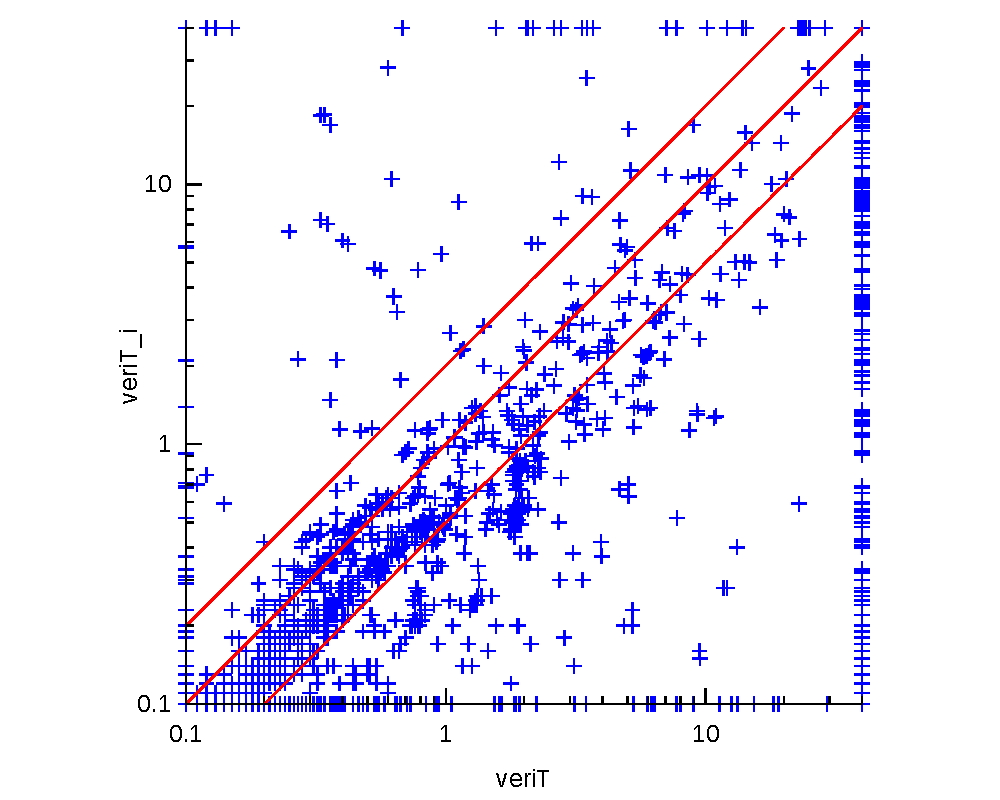
\includegraphics[scale=.35]{i_devel.pdf}
%   \caption{Impact of indexing + CCFV}
%   \label{fig:sfig1}
% \end{subfigure}%
% \hfill
% \begin{subfigure}{.33\textwidth}
%   \centering
%   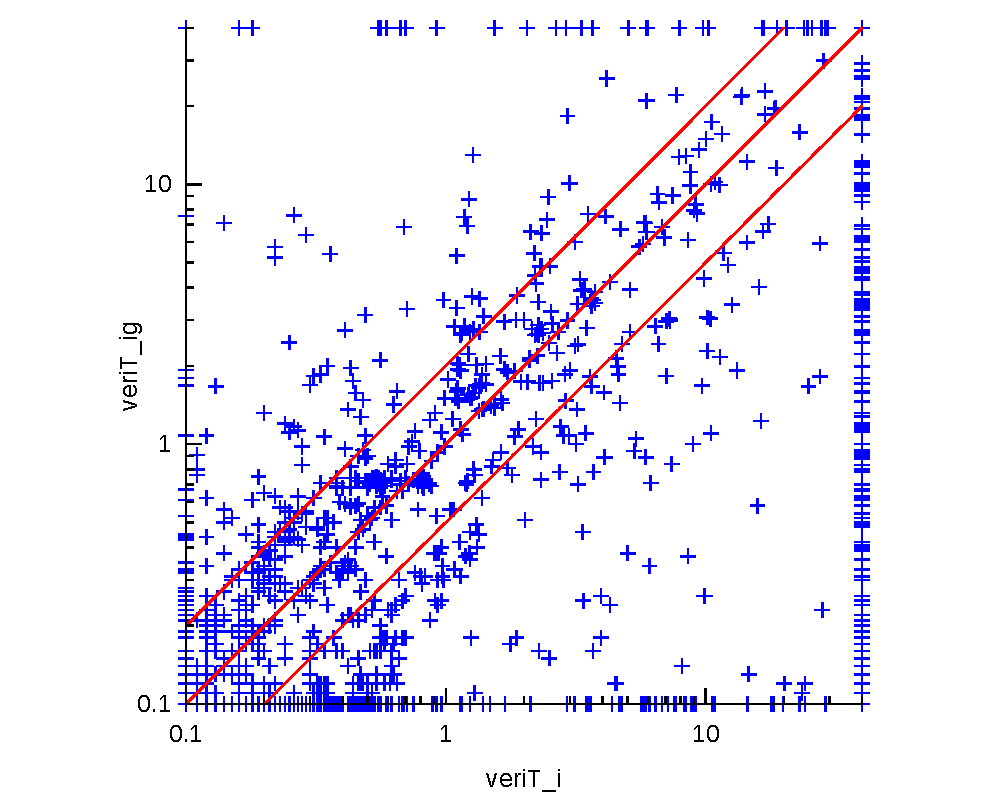
\includegraphics[scale=.35]{SIG_i.pdf}
%   \caption{Impact of goal-oriented search}
%   \label{fig:sfig2}
% \end{subfigure}
% \hfill
% \begin{subfigure}{.33\textwidth}
%   \centering
%   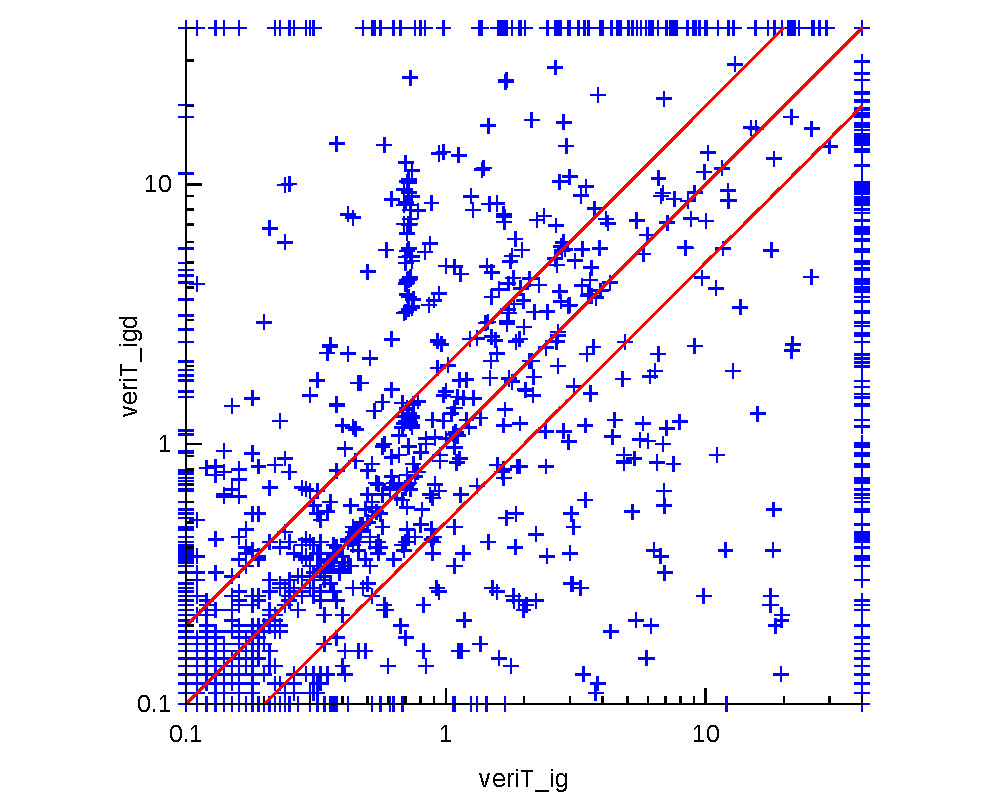
\includegraphics[scale=.35]{del_SIG.pdf}
%   \caption{Indexing}
%   \label{fig:goal}
% \end{subfigure}
% \caption{Comparisons of new indexing, CCFV and goal-oriented search}
% \label{fig:fig1}
% \end{figure}

\begin{figure}[htbp]
\begin{subfigure}{.49\textwidth}
  \centering
  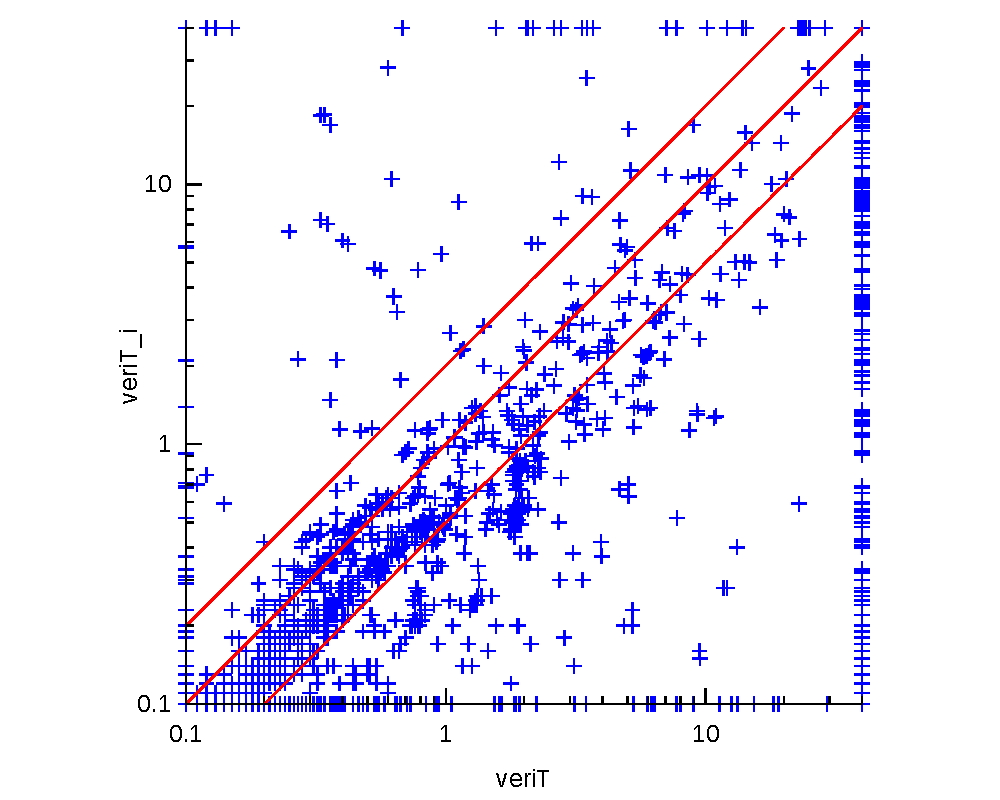
\includegraphics[scale=.42]{i_devel.pdf}
  \caption{Impact of indexing + CCFV}
  \label{fig:sfig1}
\end{subfigure}%
\hfill
\begin{subfigure}{.49\textwidth}
  \centering
  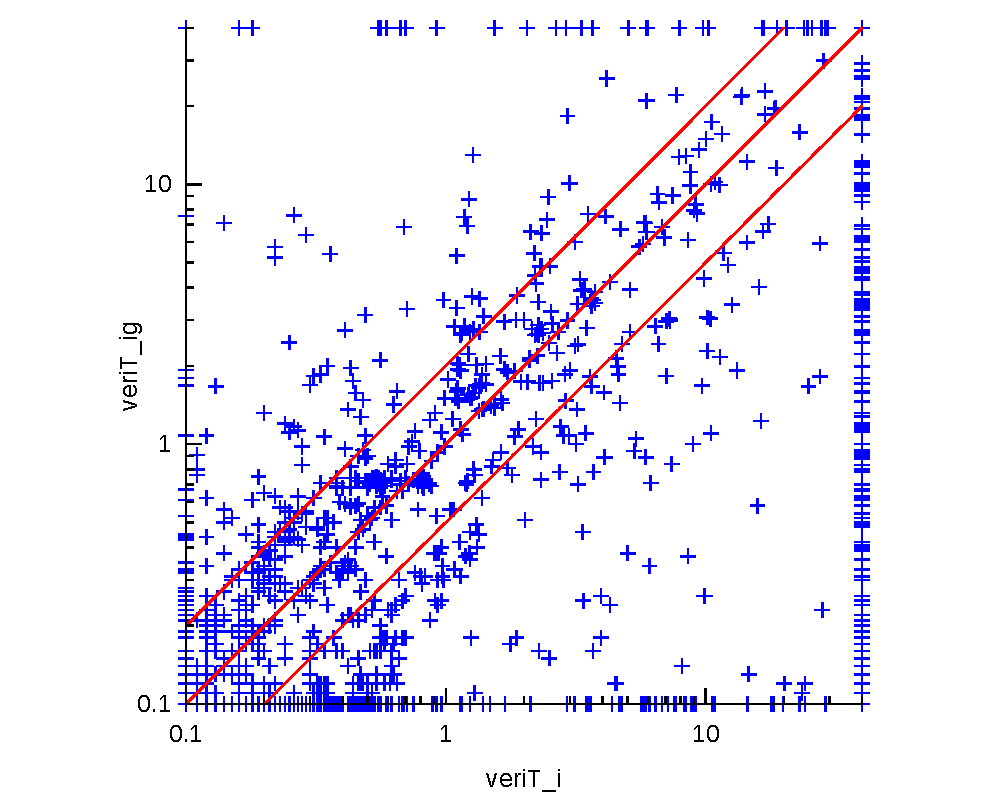
\includegraphics[scale=.42]{SIG_i.pdf}
  \caption{Impact of goal-oriented search}
  \label{fig:sfig2}
\end{subfigure}
\caption{Comparisons of new term indexing, CCFV and goal-oriented search}
\label{fig:fig1}
\end{figure}


We have also also evaluated our new implementations against the SMT
solvers \textsc{Z3}~\cite{deMoura2008-z3} (version 4.4.2) and
\textsc{CVC4}~\cite{Barrett2011} (version 1.5), both based on
instantiation for handling quantified formulas. The results are
summarized in Table~\ref{tab:comparison}, excluding categories whose
problems are trivially solved by all systems, which leaves $8,701$ for
consideration. \textsc{CVC4} solves more problems, being the more
robust SMT solver for instantiation and also applying a goal-oriented
search for conflicting instances. Both configurations of {\verit}
solve approximately the same number of problems of \textsc{Z3},
although mostly because of the better performance on the
\emph{sledgehammer} benchmarks, which have less theory symbols. There
are 124 problems solved by {\verit}+igd that neither \textsc{CVC4} nor
\textsc{Z3} solve, while {\verit}+ig solves 115 that neither of these
two do.

% [TODO] have it is cvc4, z3, me (del, sig, ...)
\begin{table}[htbp]
  \centering
  \begin{tabular}{|l|l|l|l|l|l|l|}
    \hline
    Logic & Class & CVC4 & Z3 & veriT+igd & veriT+ig \\
    \hline
    \multirow{2}{*}{UF}&grasshopper&410&418&431&\textbf{437}\\
          &sledgehammer&\textbf{1412}&1249&1293&1272\\
    \hline
    UFIDL&all&61&\textbf{62}&56&58\\
    \hline
    \multirow{5}{*}{UFLIA}&boogie&841&\textbf{852}&722&681\\
          &sexpr&15&\textbf{26}&15&7\\
          &grasshopper&320&341&356&\textbf{367}\\
          &sledgehammer&\textbf{1892}&1581&1781&1778\\
          &simplify&770&\textbf{831}&797&803\\
          &simplify2&2226&\textbf{2337}&2277&2298\\
    \hline
    \multicolumn{2}{|c|}{Total}&\textbf{7947}&7697&7727&7701\\
    \hline
    % \multirow{AUFLIRA}&&&&&&&\\
    % \hline
  \end{tabular}

  \caption{Comparison between instantiation based SMT solvers on the SMT-LIB}
  \label{tab:comparison}
\end{table}

We can see in Figure~\ref{fig:fig2} how the better {\verit}
configuration, with the goal oriented search and ``deletion'',
performs against the other solves. There are many problems which are
solved exclusively by each system, which indicates the benefit of
combining all the systems in a portfolio when trying to solve a
particular problem: while \textsc{CVC4} alone solves $\sim 92%$ of the
considered problems in 30s, by giving each of the four compared
systems 7 seconds is enough to solve \red{$\sim 97%$}\footnote{There is
  something wrong with my script.} of them.

\begin{figure}[htbp]
\begin{subfigure}{.49\textwidth}
  \centering
  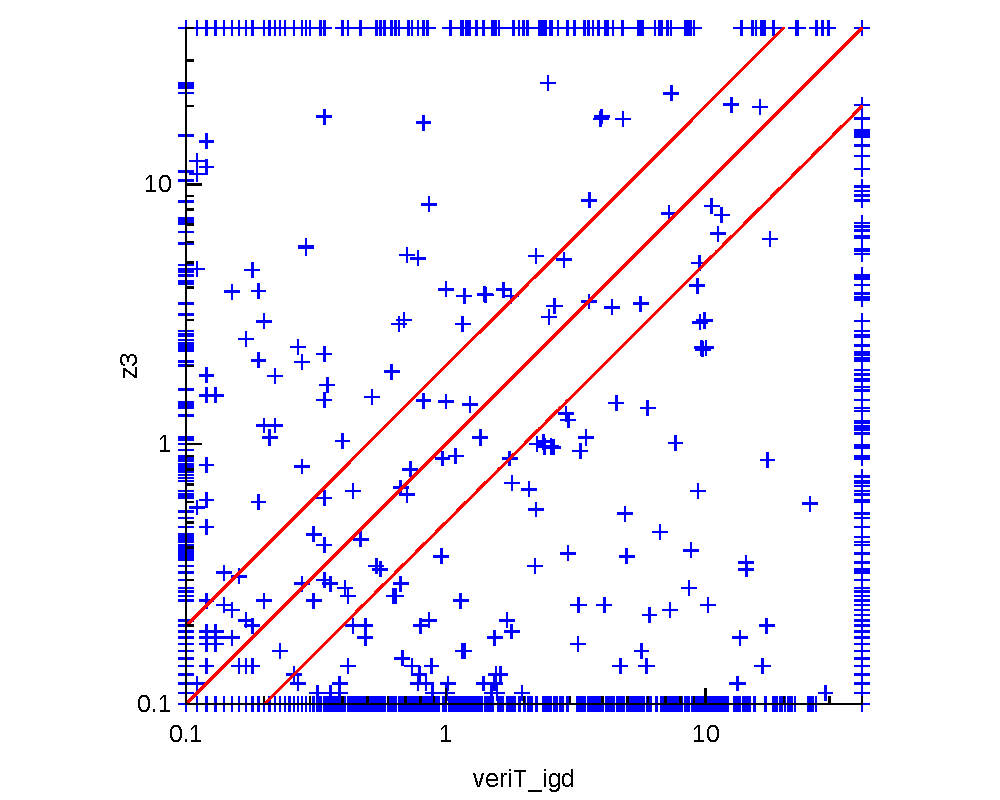
\includegraphics[scale=.42]{z3_del.pdf}
  \caption{Indexing}
  \label{fig:sfig3}
\end{subfigure}%
\hfill
\begin{subfigure}{.49\textwidth}
  \centering
  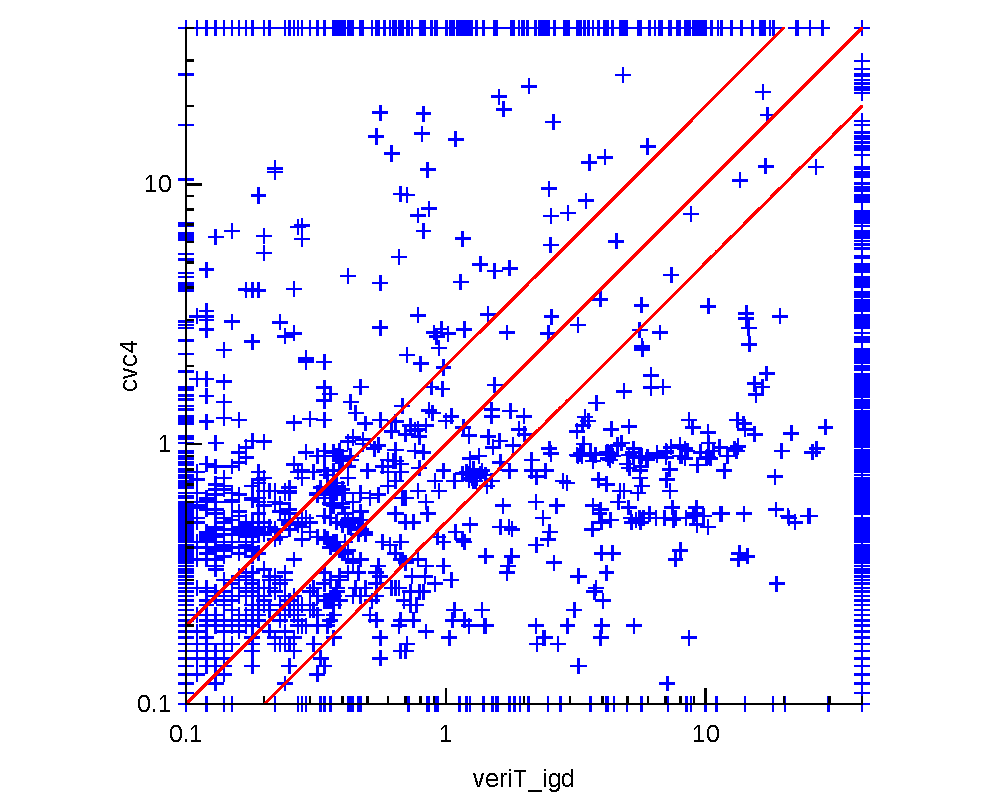
\includegraphics[scale=.42]{cvc4_del.pdf}
  \caption{1b}
  \label{fig:sfig4}
\end{subfigure}
\caption{Comparisons with SMT solvers}
\label{fig:fig2}
\end{figure}

\section{Conclusion and future work}
\label{sec:conclusion}

\begin{itemize}
  \item Better indexing (fingerprint for term indexing, discrimination trees for trigger
  insts)
  \item Incrementality
  \item Complete goal-oriented technique (connection calculus,
  rewriting, superposition with rigid variables)
  \item Build an efficient portfolio combination for maximize the
  several different parameters
\end{itemize}


\paragraph{Acknowledgements} I would like to thank my supervisor
Pascal Fontaine for all the help throughout the development of this
work.

\bibliographystyle{abbrv}
\bibliography{bib}

\end{document}

%%% Local Variables:
%%% mode: latex
%%% TeX-master: t
%%% End:

\message{ !name(main.tex) !offset(-565) }
